\documentclass[twocolumn]{article}


% Packages for formatting and settings
\usepackage[utf8]{inputenc}
\usepackage[T1]{fontenc}
\usepackage{geometry}
\usepackage{lipsum} % For dummy text, you can remove this in your actual paper
\usepackage{natbib}
\usepackage{graphicx}
\usepackage{authblk}

% Title and authors
\title{Heavenly Insights from Heavenly Words: Word Frequency Analysis on Marriage and Family Articles}
\author[1]{Weston Smith}
\affil{wms29@byu.edu}
% \affil[2]{Co-author's Affiliation, Co-author's Email}

\date{\today}

% Document begins
\begin{document}

\newcommand{\church}{The Church of Jesus Christ of Latter-day Saints }

\maketitle

\begin{abstract}
    % Your abstract here
    The Church of Jesus Christ of Latter-day Saints places supreme importance on the family. 
    It teaches that we are all family and children of God, also referred to as Heavenly Father. This then leads to the teaching that we are all brothers and sisters in God. This is further emphasized by the teaching that the nuclear family is ordained of God and that every married couple should strive to have and raise children in the covenant. A major facet of this is the emphasis on marriage. Marriage is taught as a necessary prerequisite to starting a family, and it is seen as taboo and "sinful" to engage in premarital sexual relations. Marriage is taught as an eternal concept, meaning that through a special ritual, referred to as the Temple Sealing, a couple may live together as a couple even after death. 
    This is seen in contrast to the classic position of most marriages and the vow "Til death do us part."

\end{abstract}

\section{Background}
% Your introduction here
The Church of Jesus Christ of Latter Day Saints place supreme importance on the family. It teaches that we are all family and children of God, also referred to as Heavenly Father. This then leads to the teaching that we are all brothers and sisters in God. This is further emphasized by the teaching the nuclear family is ordained of God and that every married couple should strive to have and raise children in the covenant. A major facet of this the empaphasis on marriage. Marriage is taught as a necessary prerequisite to starting a family and it is seen as taboo and "sinful" to engage in premarital sexual relations. Marriage is taught as an eternal concept, that through special ritual, referred to as the Temple Sealing, a couple may live together as a couple even after death. This is seen in contrast to the classic position of most marriages and the vow "Til death do us part."

This emphasis is strongly reflected in the rhetoric and topics commonly emphasized and spoken about in General Conference. General Conference is a biannual meeting where members of the \church listen to instructions from their prophet, apostles, and other prominent church leaders. The topics for these are sometimes assigned and sometimes left up to the discretion of those who are speaking. It is an opportunity for the members to receive renewed instruction and to reconstitute their time for Jesus Christ. Such rhetoric is very different from the classic scientific and, as church leaders often say, "wordly" rhetoric.
\section{Methodology}
% Your methodology description here
Articles from these General Conferences from various times and various authors that have been self-classified by the Church administrators about "marriage" and "family" These topics are derived from the website of \church and are prescribed by those in charge of media for the church. These were then obtained by parsing all URLs on a specific page and grabbing any URL that had an article. This allowed a quick method for downloading 134 articles on marriage and 36 articles on family.

These will be compared to articles that have been chosen from Academia. In the absence of nice categories and easy access to articles, a different method had to be chosen. The method was using different keywords mixed with either "marriage" or "family." This is because marriage and family are often used in different academic disciplines to mean things other than the union of two people and a collection of humans that share special bonds.

After the articles were gathered, they were split into words. All non-alpha characters were removed, including numbers and punctuation. The words were then filtered off of a basic stop-word list. This is a list of basic words like "the," "it," and "and" that don't have much meaning to themselves. The remaining words were then counted. The articles were counted individually, and then their word counts were added together. The sixty most common words were chosen for analysis. At first, frequency compared to borer use was considered. This was decided to be uneffective because of the niche nature of both church and scholarly articles. For articles from the Church, words that only the Church uses, like "Liahona," and other words with religious significance had higher than expected ratios. The decision was made that such words corrupted raw frequency data where just a few outliers could disrupt the whole.

\begin{center}
    \parbox{\linewidth}{\centering\textbf{Example hybrid search terms}}
\end{center}

\begin{itemize}
    \item "Marriage happiness"
    \item "Marriage satisfaction"
    \item "Marriage divorce"
    \item "Marriage
    \item "Family happiness"
    \item "Family children"
\end{itemize}

This methodology allowed the collection of 25 articles: 20 about marriage and 5 about family. These articles were then parsed, and the word count was calculated. This was done by using the Python library "Beautiful Soup" to parse the HTML and then using the Python library "Natural Language Toolkit" to tokenize the words and then count them. This was then compared to the word count of the General Conference articles. The word count was then normalized by dividing the word count by the total number of words in the article. This allowed relative comparison between different articles and relative word count between scholarly and church articles. In the end, the raw frequency number wasn’t used but instead the position it was in the ranking of how common it was.

The collection of scholarly articles posed some interesting problems. One of these was my own bias in the selection and overemphasis of a topic. This happened when certain search engines and databases were used, including the Standard Database from the Brigham Young University library and the Google Scholar search engine. This is because there were large clusterings on certain topics that were determined to pose a danger to the results. For example, there was a dearth of articles about gay marriage; such articles would have different subjects than articles about marriage and the family in other contexts and would often focus on legislative challenges instead of internal challenges, including happiness and satisfaction. The call was made to limit the number of articles on the subject and to avoid using such keywords to try and find other types of articles.

\section{Results}
% Your results here
\begin{table*}[h] % [h] means 'here', allowing the table to be placed here in the document
    \centering
    \caption{Sentiment Analysis of Common Words}
    \label{tab:example}
    \begin{tabular}{|c|c|c|} % Columns are centered; use 'l' for left-aligned, 'r' for right-aligned
        \hline
        \textbf{Subject}   & \textbf{Sentiment Value} & \textbf{Sentiment Type} \\ % Header row
        \hline
        Scholary Family    & 63.1\%                   & Negative                \\ % Row 1
        \hline

        LDS Family         & 94.2\%                   & Positive                \\ % Row 2
        \hline

        Scholarly Marriage & 49.8\%                   & Negative                \\ % Row 3
        \hline

        LDS Marriage       & 88.5\%                   & Positive                \\ % Row 3

        \hline
    \end{tabular}
\end{table*}

The results of the analysis show that there is a significant difference in the words used between scholarly articles and articles of \church. Most interestingly, the difference between \church and scholarly articles is not as large as the difference between scholarly articles and scholarly articles on the same subject, which was much greater than the difference of words between scholarly articles on different subjects or articles from \church on different subjects. This shows significant differences in focus that will be analyzed later on.


This table shows a sentiment analysis of the sixty most common words for each type of article. The percent value is the confidence value that the sentiment type is correct. So there is a 63.1\% confidence that the top sixty most common words for scholarly articles have a negative sentiment. This shows a clear distinction between the sentiment of scholars and Church articles. Church articles are much more positive, while scholarly articles are much more negative.
%insert figure
\begin{figure}[h]
    \centering
    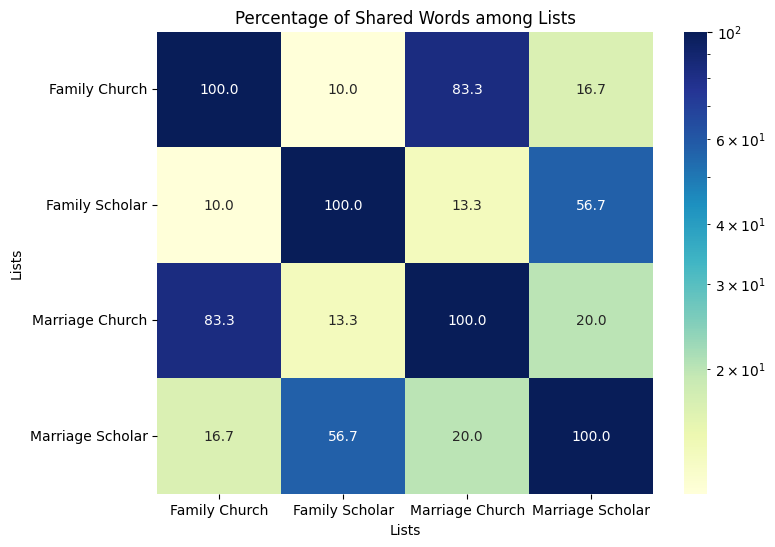
\includegraphics[width=\linewidth]{../heatmap.png}
    \caption{Heatmap of Word Frequency}
    \label{fig:heatmap}
\end{figure}

The chart shows what percentage of words the following lists have in common. From the heatmap, it is evident that Church articles share many words and scholarly articles share many words, but family and marriage articles share very few articles. This shows that scholarly articles think about marriage and family as very similar and approach them very similarly, while Church articles think about marriage and family as very different and approach them very differently.

% Your discussion here


%insert figure
\begin{figure}[h]
    \centering
    \rotatebox{270}{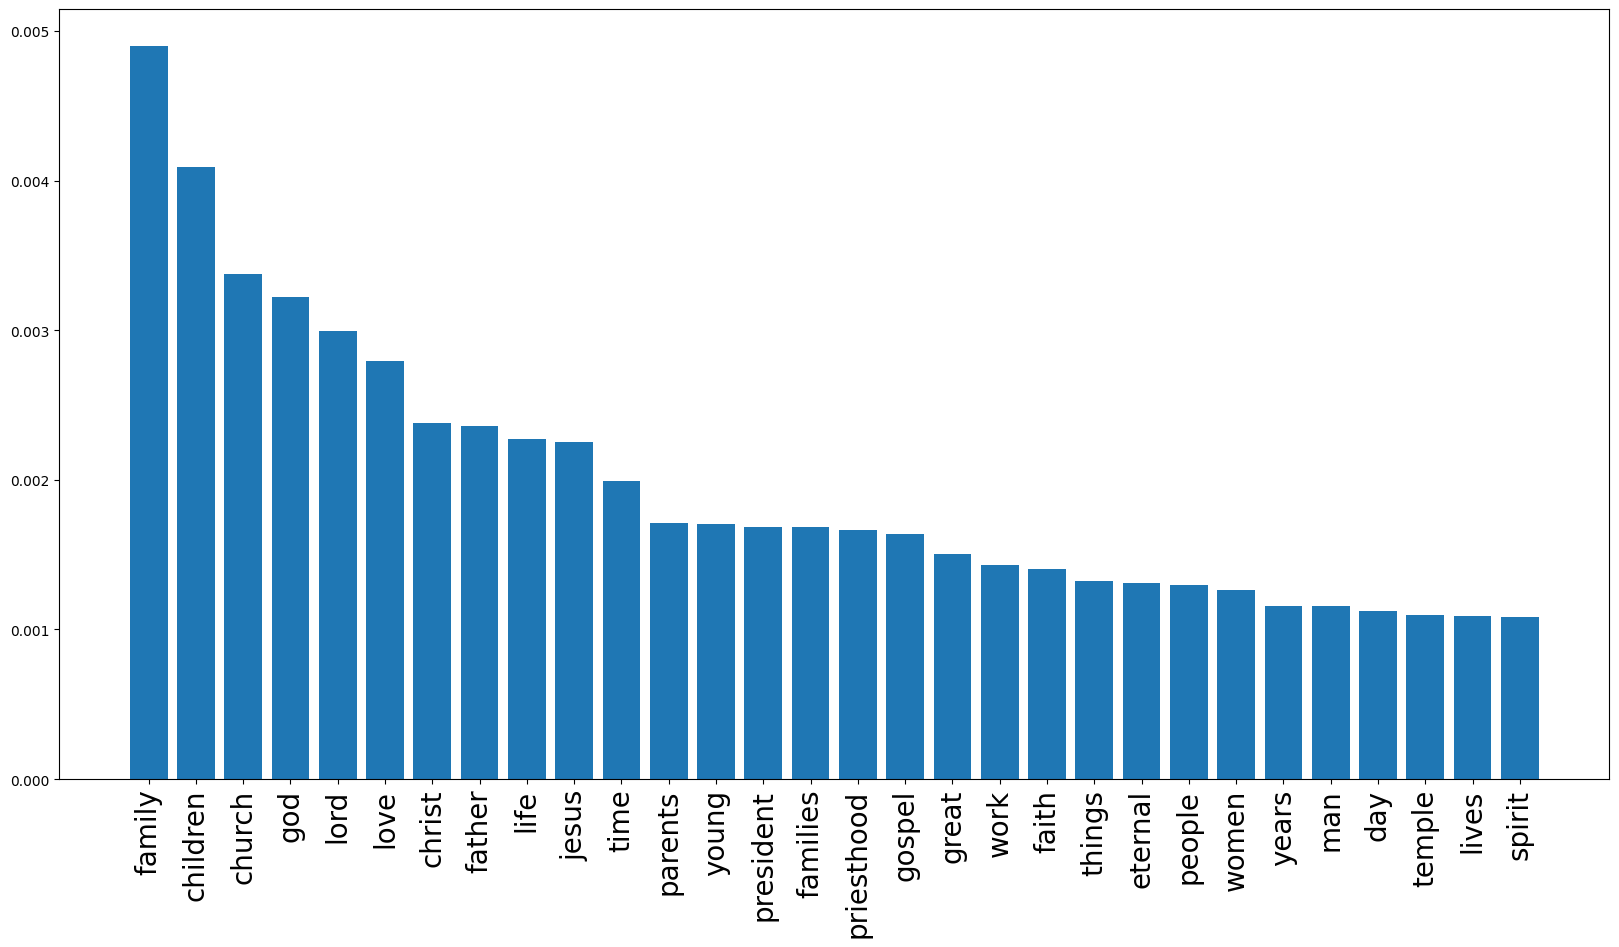
\includegraphics[width=1.5\linewidth]{../fc_wc.png}}
    \caption{30 Most Common Words in Family Church Articles}
    \label{fig:fcwc}
\end{figure}



%insert figure
\begin{figure}[h]
    \centering
    \rotatebox{270}{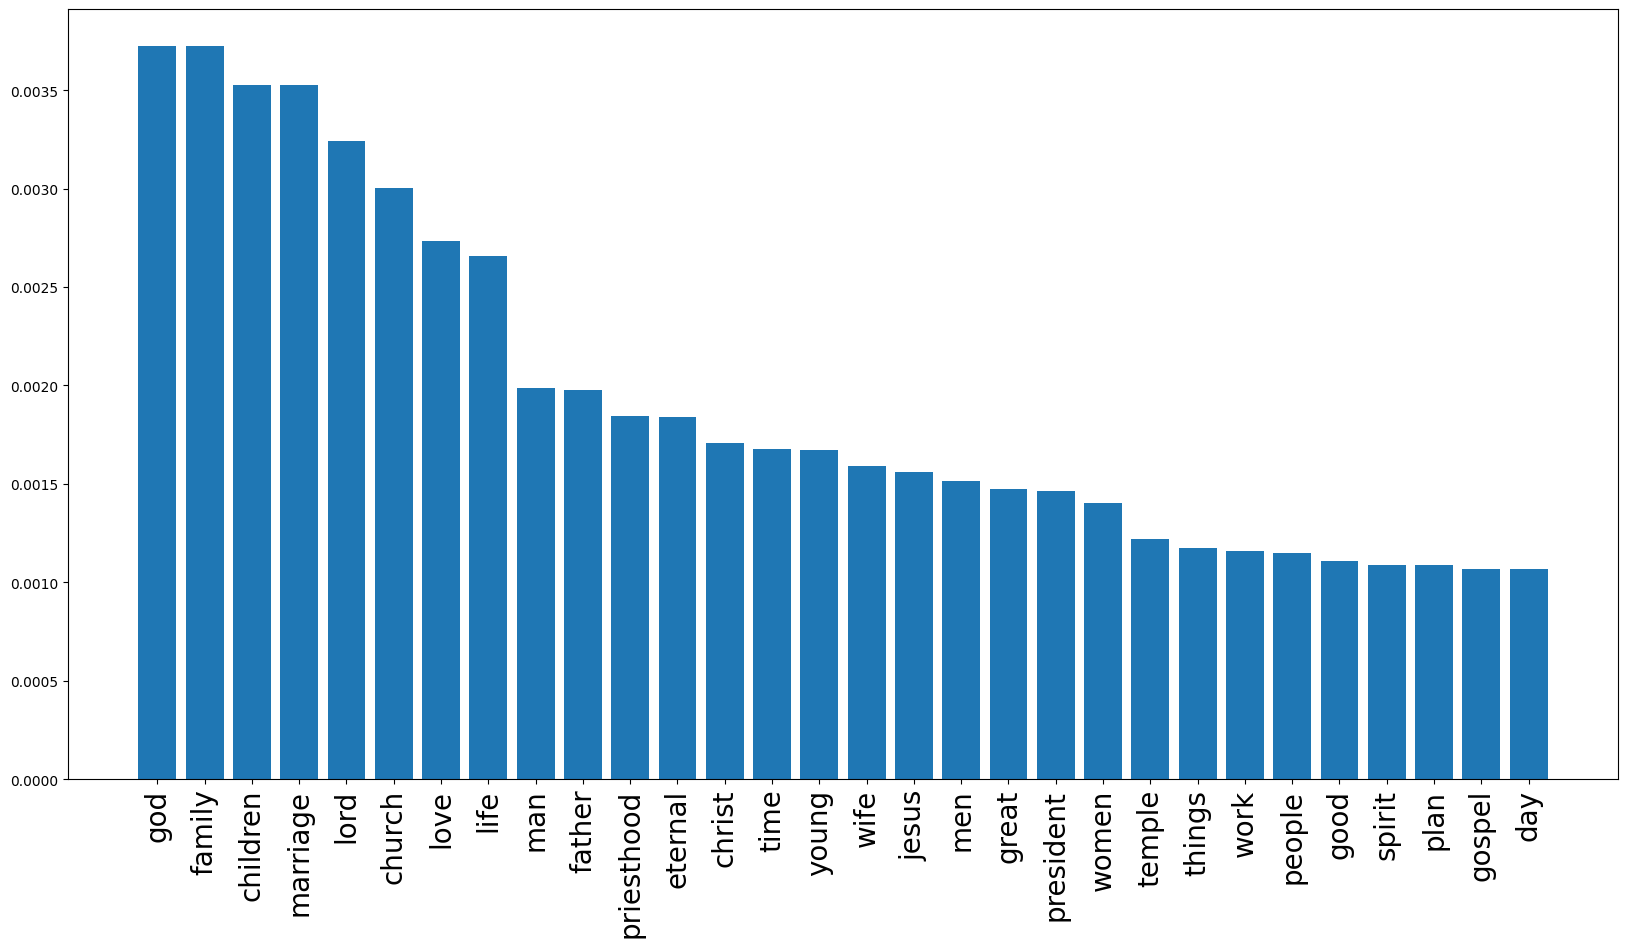
\includegraphics[width=1.5\linewidth]{../mc_wc.png}}
    \caption{30 Most Common Words in Marriage Church Articles}
    \label{fig:mcwc}
\end{figure}

The plots for family and marriage church articles both have very similar words, as described above. Even in the word count of marriage articles, family and children rank higher than marriage. This is indicative of the incredible emphasis church leaders put on having children in family bonds when discussing marriage. Specific words will be explored more. Religious words like "temple," "Jesus," and "gospel" are also common in both. This is to be expected from religious articles.%insert figure

\begin{figure}[h]
    \centering
    \rotatebox{270}{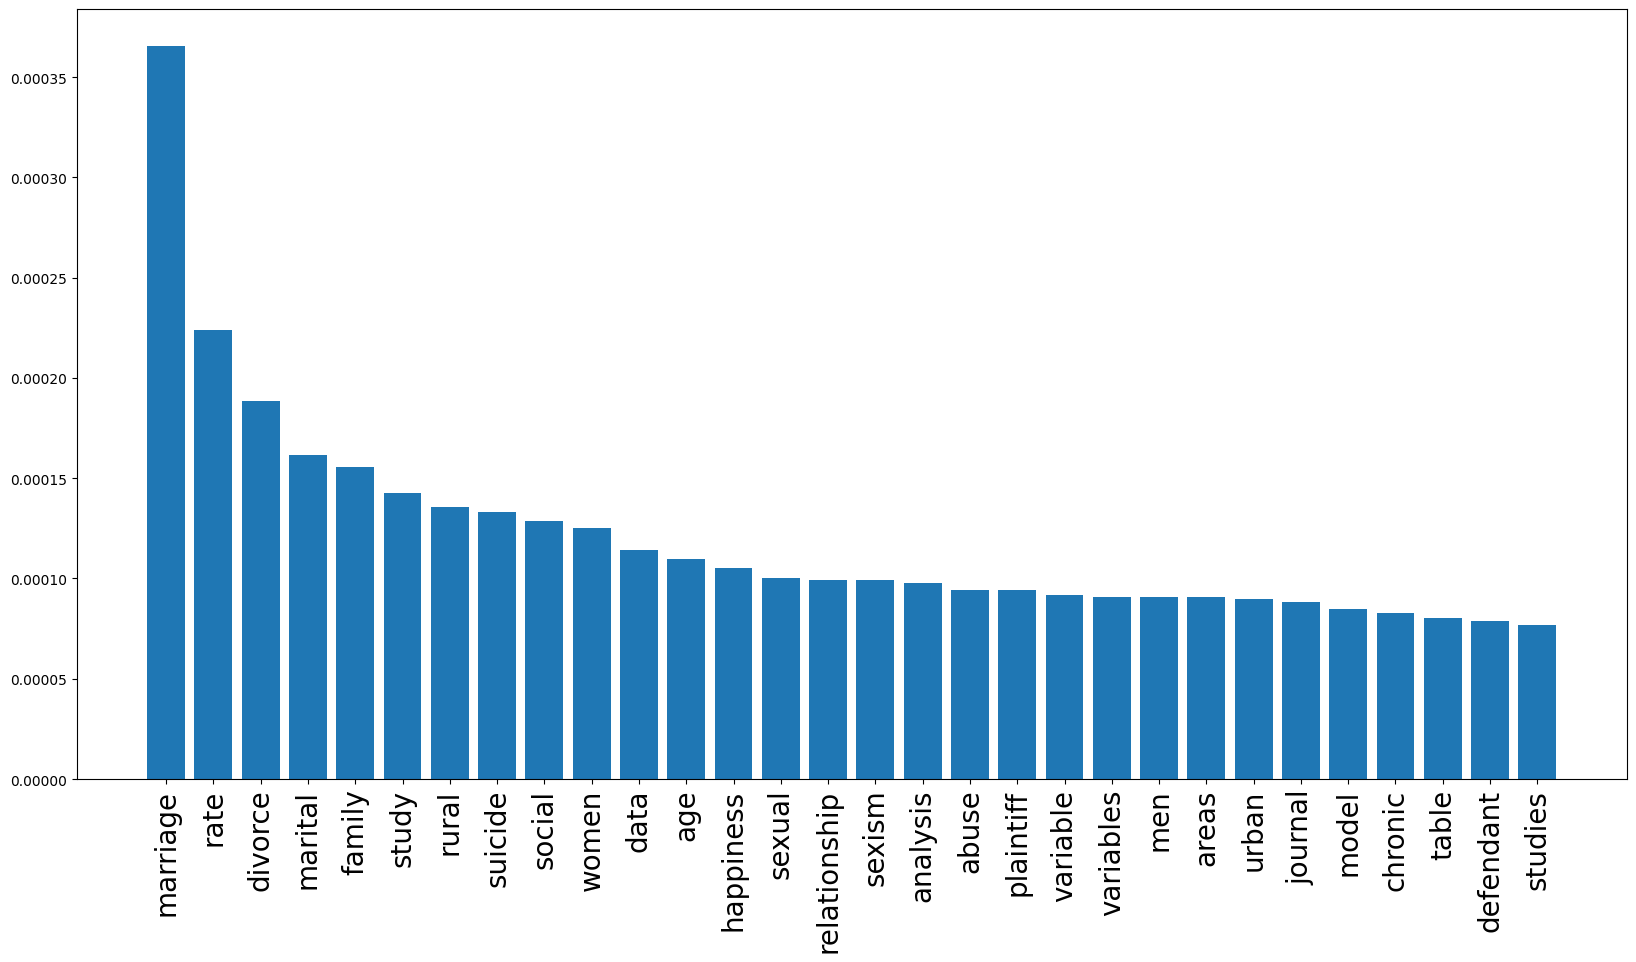
\includegraphics[width=1.5\linewidth]{../fs_wc.png}}
    \caption{30 Most Common Words in Family Scholarly Articles}
    \label{fig:fswc}
\end{figure}

%insert figure
\begin{figure}[h]
    \centering
    \rotatebox{270}{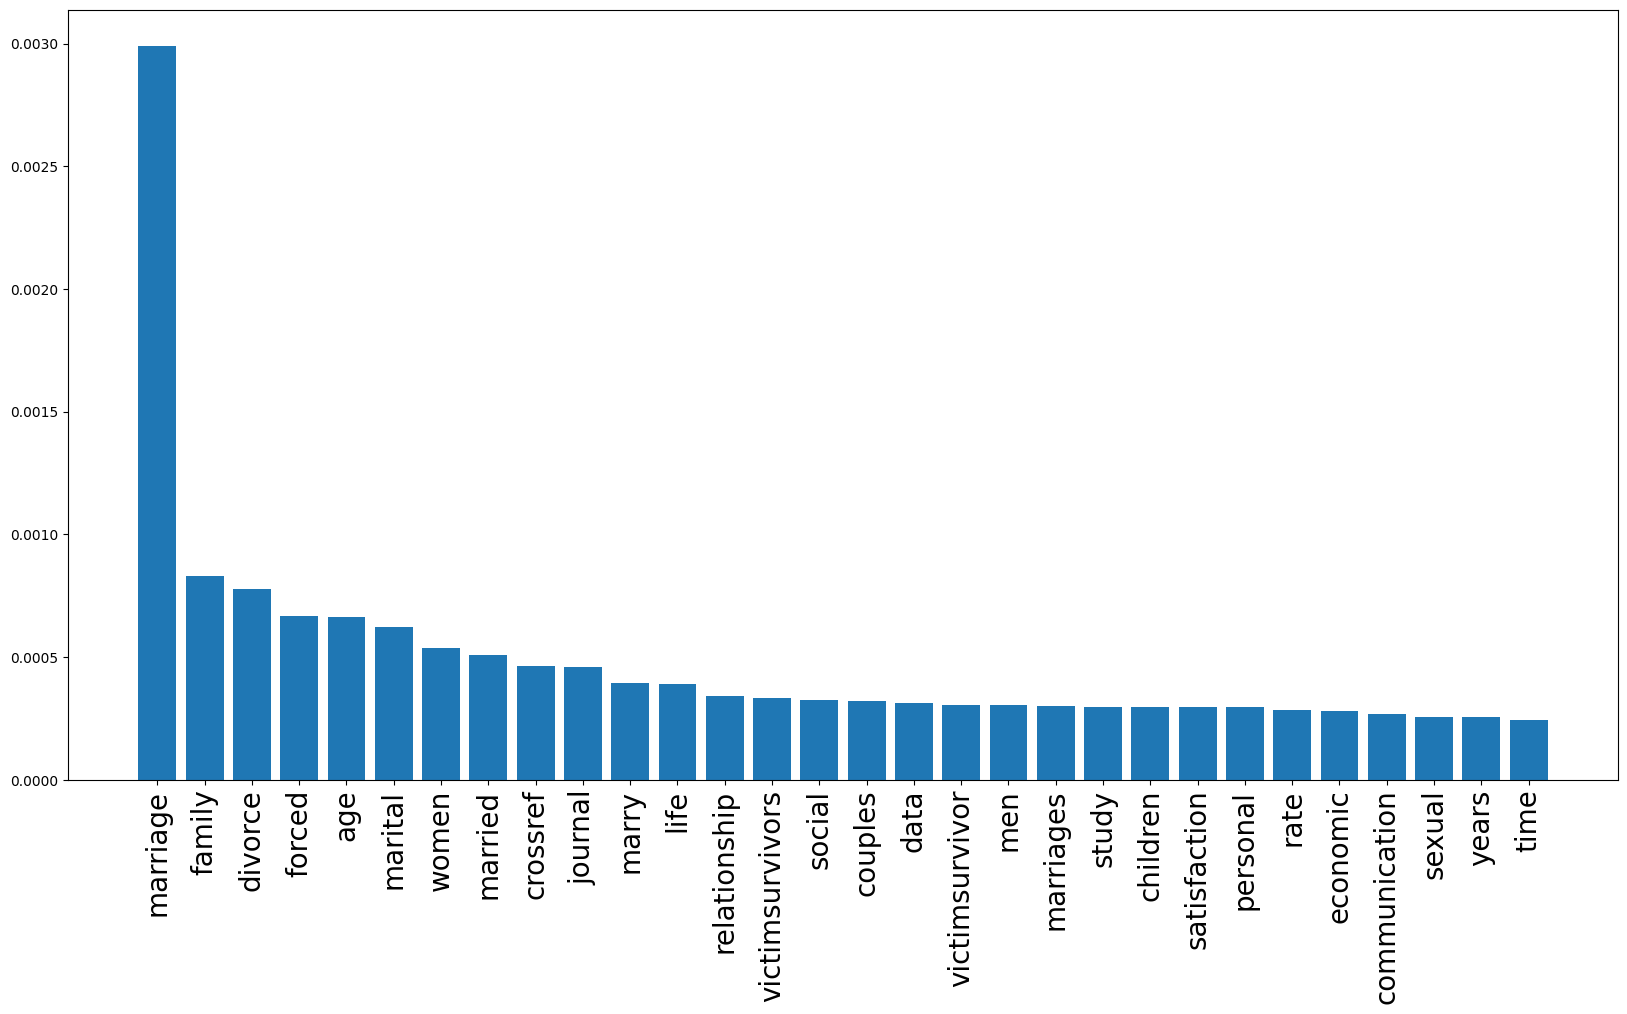
\includegraphics[width=1.5\linewidth]{../ms_wc.png}}
    \caption{30 Most Common Words in Marriage Scholarly Articles}
    \label{fig:mswc}
\end{figure}

The scholarly tone can easily be derived from some of the more scientific words used in the scholarly articles that show up in the most common word lists. This includes words such as "rate," "social," "rural," and "model." Another interesting inclusion in both scholarly lists is the word "divorce," which is absent from both other lists.

\section{Analysis}

Certain words have a different meaning and subtext in these specific contexts. This allows us to analyze individual words and how they are used in order to find some of the meaning in these texts. Words like marriage are used differently in the scholarship versus the church articles. An analysis of these words will follow.
\subsection{Divorce}

One of the most interesting omissions from the word list of common words from articles from \church is the word divorce. The word divorce is incredibly common in both the family and marriage scholarly articles. Some things can be garnered from this difference in frequency in these articles. This analysis will include plenty of conjecture and hypothesis. First, the scholarly view of divorce is what happens to couples when things go badly. In the scholar's mind, the solution to marital problems. This shows that divorce is always an easy option for a couple. One could also surmise that divorce is seen as an inevitable for some couples that cannot be changed.

This cannot be more different to the approach of \church. The exclusion of the word divorce from the frequency list can be seen as the word divorce not even being in the vocabulary of the church. Divorce is not seen as a "get out of jail free card". Divorce is not considered something common and not considered a solution to problems. In the church, marriage is seen as eternal and this gives it an added sense of worth. Marriage is something special that should not be touched. It is something this will go on after life and should be treated as such. Marriage is holy and ordained of God, it is worth it to push forward and work through the marital problems to avoid divorce. This just shows completely divergent strategies in dealing with marital problems and divorce.

\subsection{Time}

Time appears in both the scholary and church articles. Though it is very common in both the family and marriage sections. This emphasis on time is often used in advice for families in general. It is the suggestion that family and marriage is something that must have our focus and time. It shows us that we need to work on our family and marriage and spend time on it. We cannot be idle and just sit around and hope things will turn out well. This also leads into the religious words used in the church articles. Time should be spent on nurturing children in the gospel. Time needs to be spent working on ones family and only through this time and effort spent can the family be strengthend.

\subsection{Forced}


The negative language from the scholarly articles is very telling of the attitude and focus of such articles. This is especially seen in the word "forced". The word forced is in reference to forced marraiges, where on of the members of the marriage didd not have a choice in the matter.
The scholarly articles also focus on many other negative trends in marriage or negative consequences of some marraiges including "risk", "", "abuse", and

\subsection{God}

God is a central element of the discussion of dialogue regarding any topic in \church. This is readily apparent in the church articles about marriage, where God is more common than any other word. This shows that the church teaches that by focusing on God, marriages can be improved. This means that when a couple is trying to become closer, growing closer to God allows this to happen. When God is the focus of people's lives, it allows other problems to move out of the way. When we focus on God, we can overcome any simple things that people face in a marriage environment. This is one of the key elements that allows no focus on divorce to exist in church articles.

\section{Conclusion}
% Your conclusion here

The study conducted a comprehensive word count analysis to compare articles on marriage and family from scholarly sources and those originating from \church. The results highlighted distinct differences in word usage, sentiment, and thematic emphasis between the two types of articles. Notably, scholarly articles displayed more negative sentiments and focused on topics such as divorce, forced marriages, and risk, while articles from \church  exhibited a more positive sentiment, emphasizing the importance of marriage, family, and God's role in strengthening familial bonds. This research contributes to understanding the varying perspectives on marriage and family, providing insights into how different contexts shape discourse surrounding these fundamental societal institutions.

% References/Bibliography
% \bibliographystyle{plainnat}
% \bibliography{references} % Replace 'references' with your actual .bib file name

\end{document}
